% !TeX spellcheck = it_IT

\section{Wireless Local Area Network WLAN}
Lo standard considerato da adesso è 802.11. I requisiti generali sono: 
\begin{itemize}
	\item Throughput maggiore possibile
	\item elevato numero di nodi, gestiti da più celle
	\item connessione verso la dorsale (backbone) cablata
	\item Raggio 100-300m
	\item Utilizzo efficiente (non estremo) della batteria
	\item Più WLAN devono poter coesistere
	\item Operare nelle bande di frequenza unlicensed
	\item Configurazione dinamica (selezione canali, autenticazione)
\end{itemize}

\paragraph{Wireless Fidelity WiFi:} Si ha una rete con \textbf{uno o più Access Point AP}, coordinata da \textbf{Point Coordination Function PCF} (ovvero si ha un solo punto di coordinamento, l'AP). Un \textbf{Basic Service Set BSS} identifica la cella o rete WiFi (nome/caratteristiche della rete).
\begin{center}
	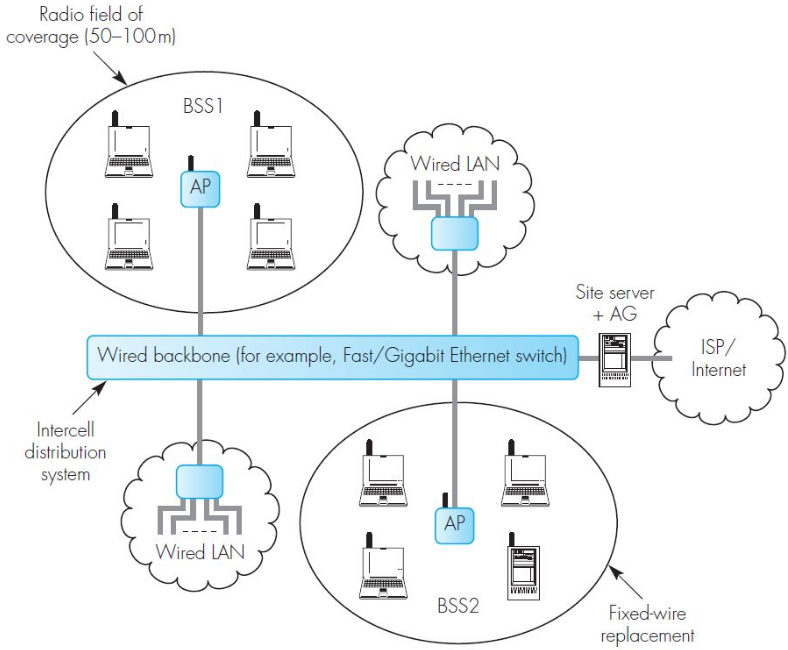
\includegraphics[width=0.7\linewidth]{img/wlan/wifistruct1}
\end{center}

\newpage

Si può anche avere una \textbf{rete Ad-Hoc}, senza una PCF, ma con una \textbf{Distributed Coordination Function DCF}, con un \textbf{Independent Basic Service Set IBSS}
\begin{center}
	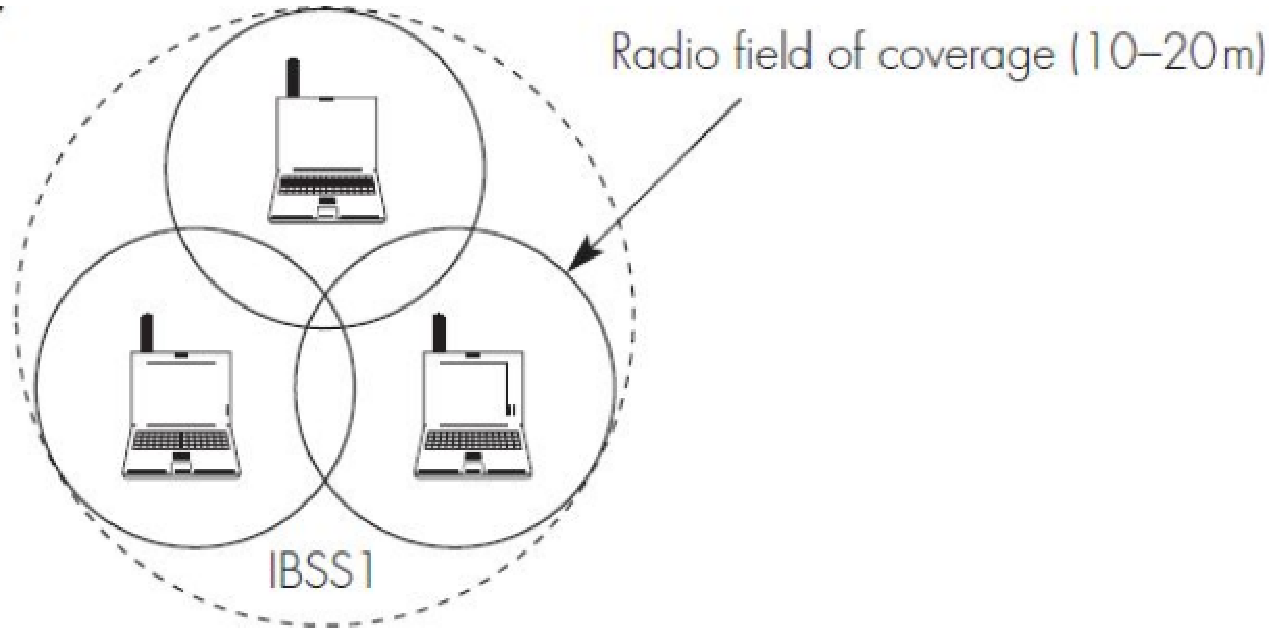
\includegraphics[width=0.45\linewidth]{img/wlan/wifistruct2}
\end{center}

\paragraph{Architettura dei protocolli:} 
\begin{center}
	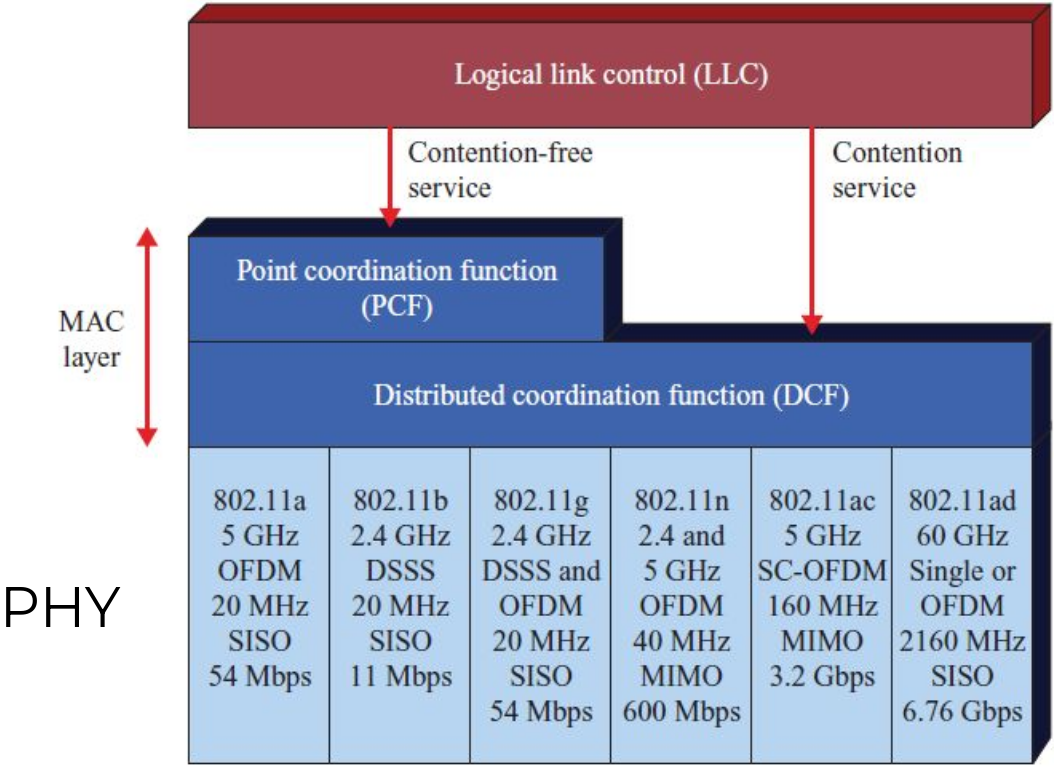
\includegraphics[width=0.75\linewidth]{img/wlan/protarch1}
\end{center}
Mostrate in ordine da sinistra a destra, a livello fisico ci sono le versioni di WiFi, anche se l'ultimo rappresentato non è WiFi 6 (quello è 802.11ax). Sopra c'è il livello MAC, poi il Logical Link Control che permette di avere servizi. \\

%Tabella? s7
Il throughput diverso (visibile \href{https://en.wikipedia.org/wiki/IEEE_802.11#Protocol}{\texttt{in questa tabella}}) è determinato da dimensione del canale, aumentata nel tempo, frequenze utilizzate, modulazioni con più bit per symbol e MIMO (Multiple Input Multiple Output, fino a 16 antenne diverse per fare input/output).\\

\newpage

\paragraph{Servizi Logical Link Control LLC:} Offre principalmente tre servizi: 
\begin{itemize}
	\item \textbf{Unacknowledged connectionless service}: consegna non garantita, datagram indipendenti, senza controllo di errori o di flusso; cosa capita capita
	\item \textbf{Connection-mode service}: canale punto-punto, correzione degli errori e controllo di flusso; connessione affidabile
	\item \textbf{Acknowledged connectionless}: datagram indipendent, acknowledged datagram; senza connessione, ma con ack
\end{itemize}

\paragraph{Infrastruttura 802.11:} 
\begin{center}
	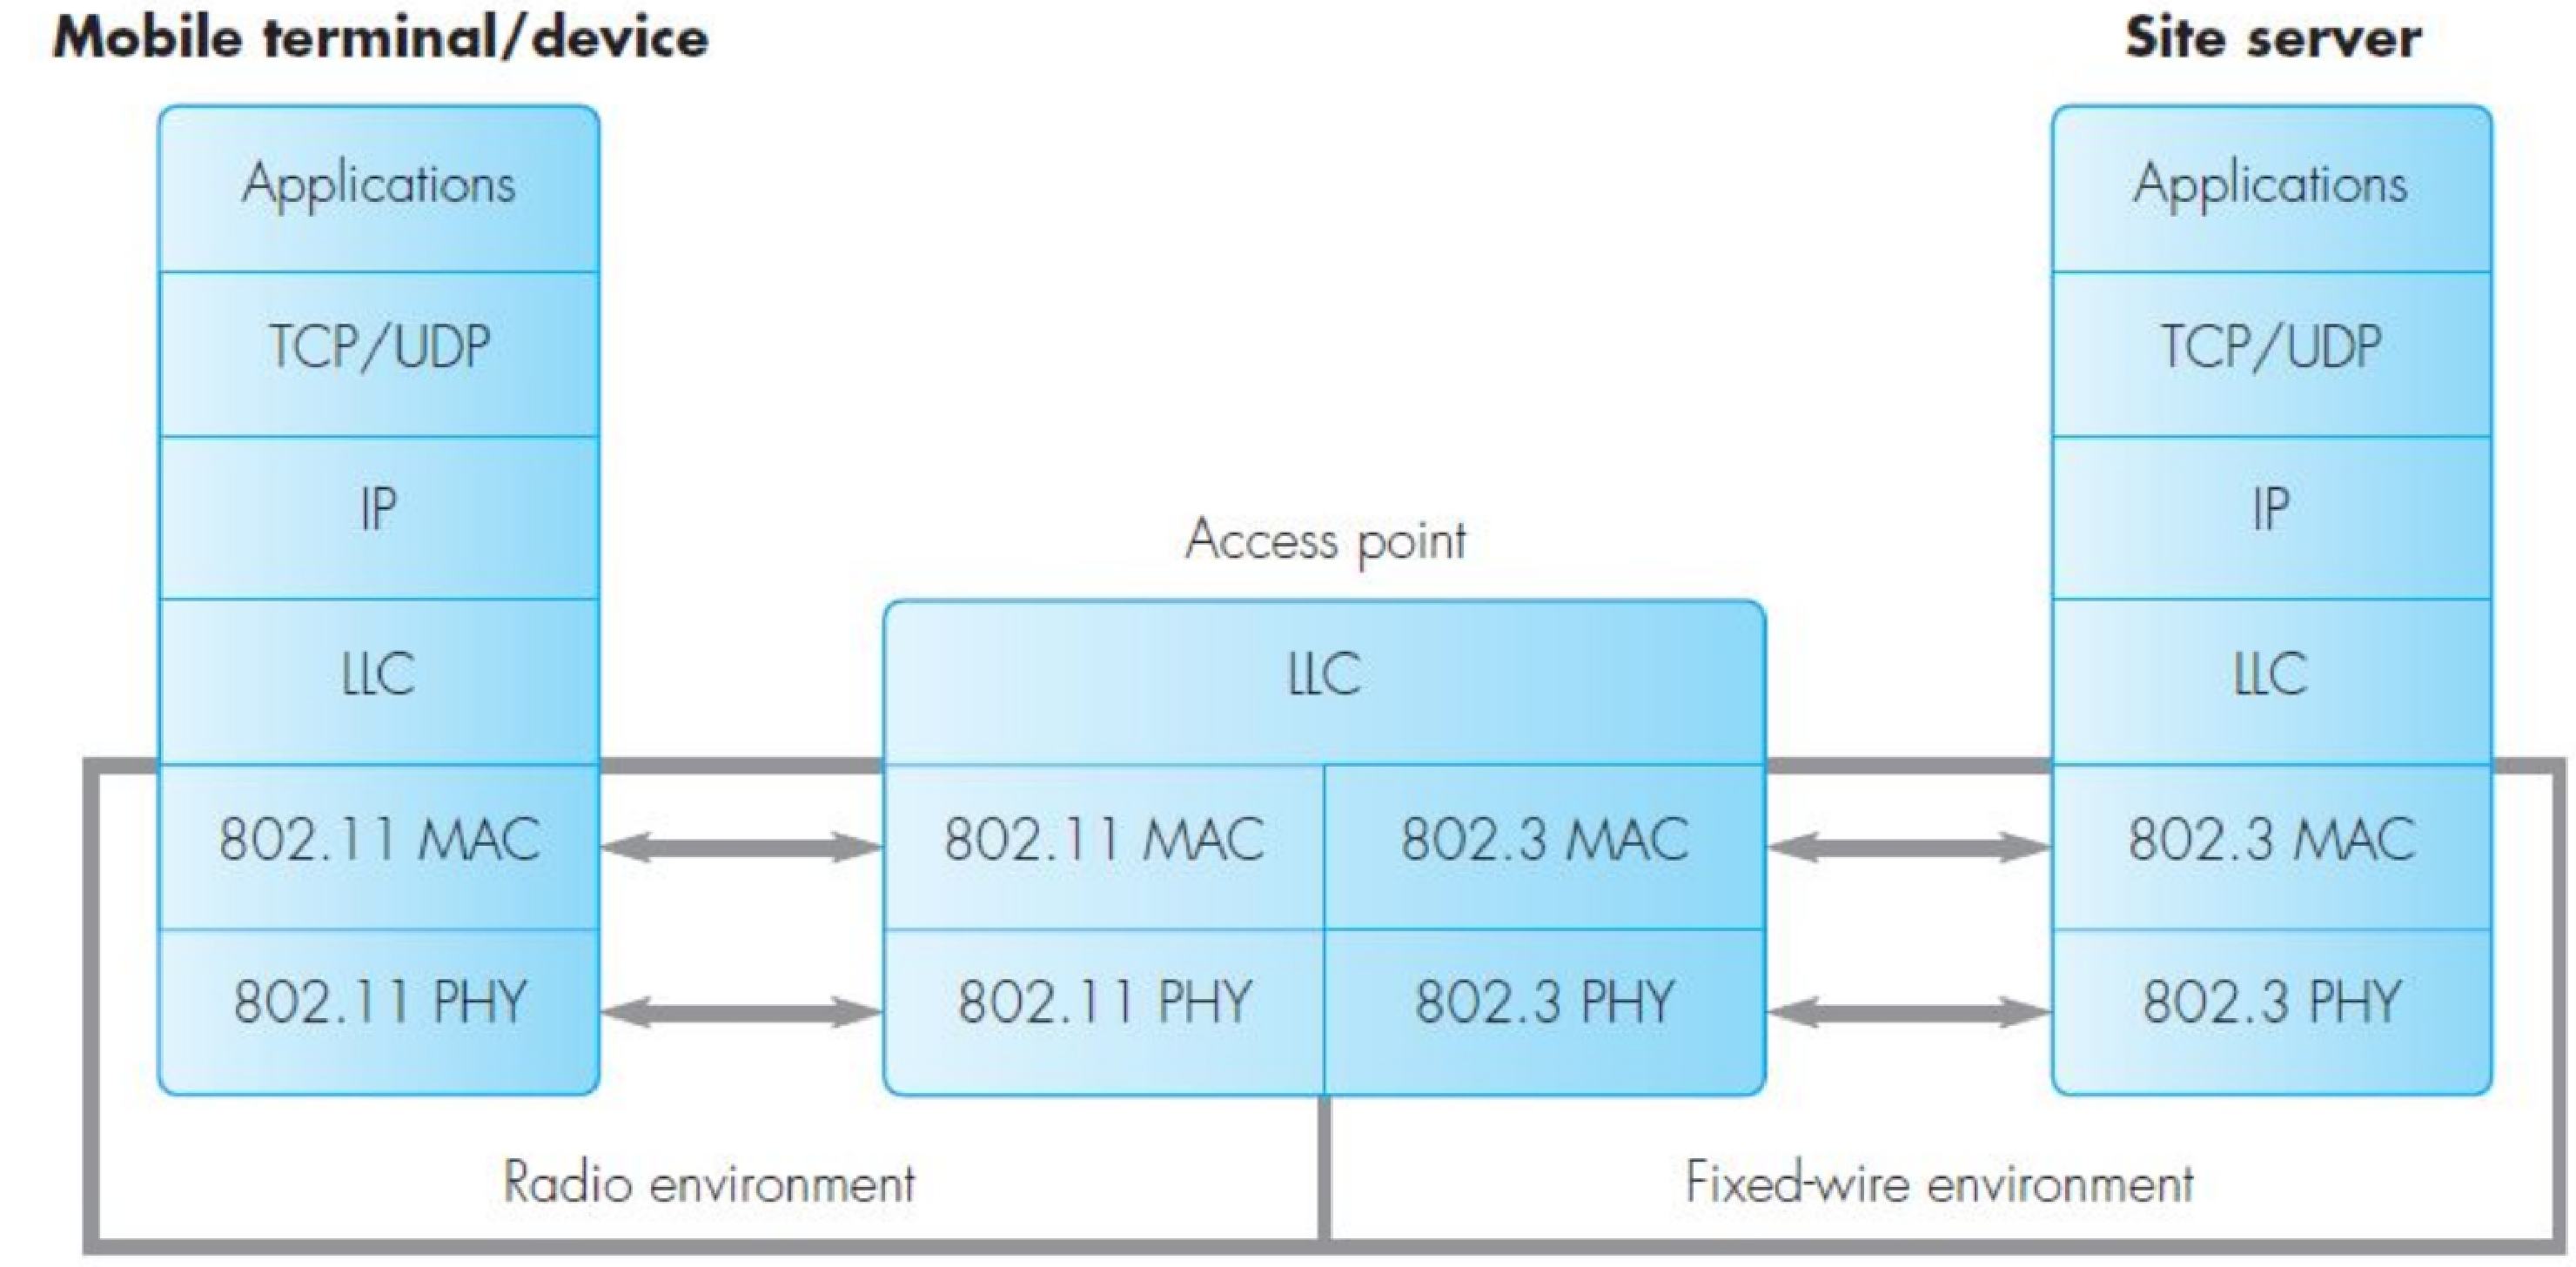
\includegraphics[width=0.85\linewidth]{img/wlan/infr}
\end{center}
Il livello LLC è comune a 802.X.  \\

\paragraph{Livelli Pacchetti:} La struttura per l'incapsulamento dei livelli è 
\begin{center}
	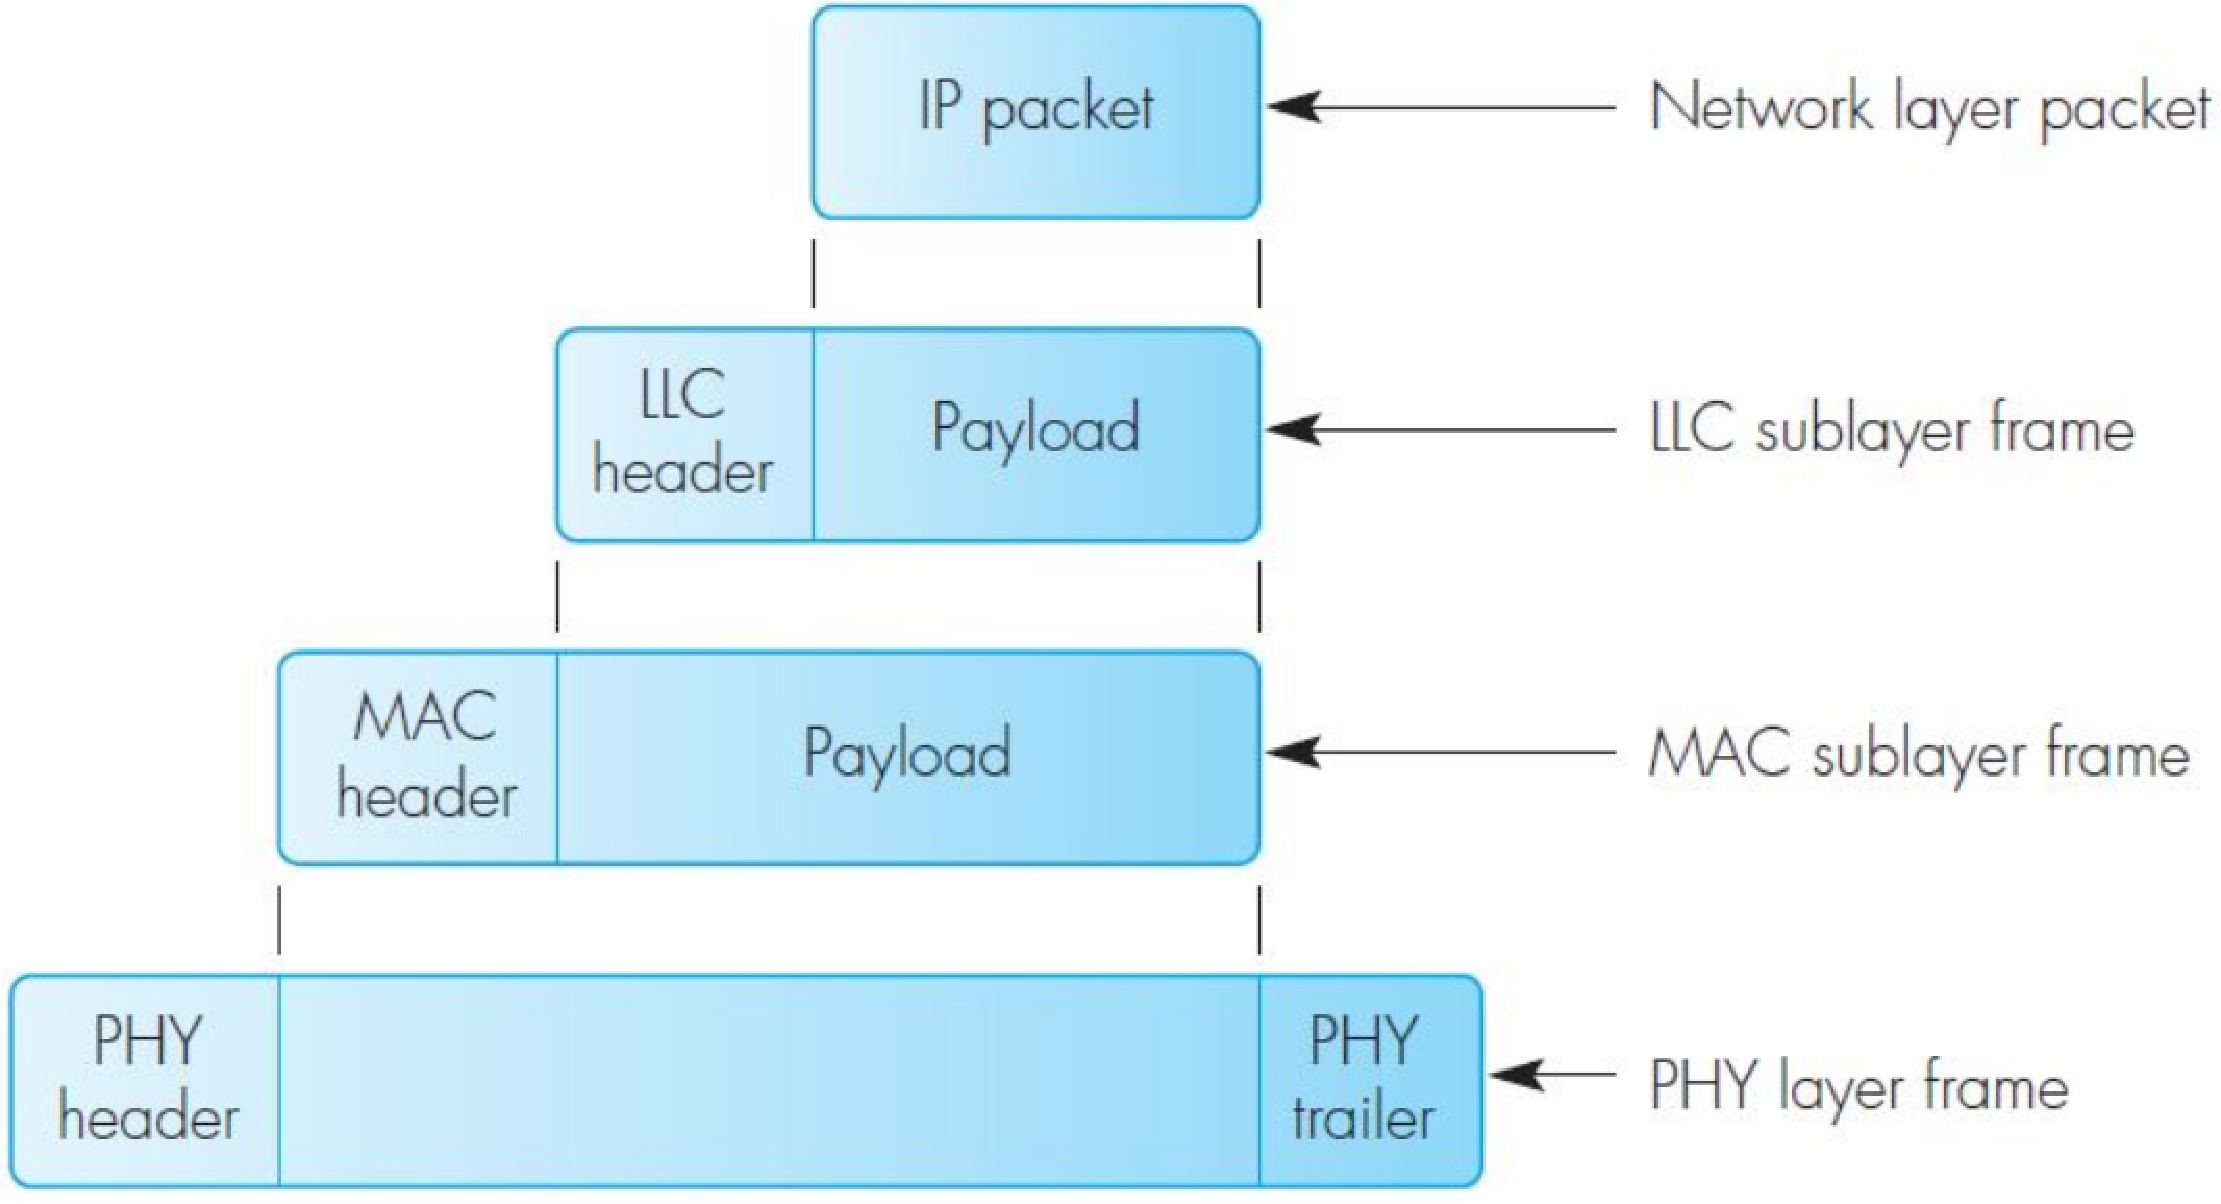
\includegraphics[width=0.6\linewidth]{img/wlan/pacch1}
\end{center}
Ovvero, fisico, MAC, LLC, poi pacchetto di rete.

\newpage

\subsection{Sottolivello MAC}

Abbiamo un canale \textit{molto} inaffidabile (rispetto ad un canale cablato), con molte informazioni da trasmettere, e di conseguenza frame più complessi (rispetto a 802.3). Il frame di MAC 802.11 ha un payload massimo di $2304B$.\\

Il sottolivello MAC offre due servizi: 
\begin{itemize}
	\item \textbf{Servizio dati asincrono}: non ha garanzie sul delay e quindi sulla QoS, best effort
	\item \textbf{Servizio time-bounded}: offre garanzie sul delay, disponibile solo in presenza di un coordinatore (AP)
\end{itemize}

\subsubsection{Distributed Coordination Function DCF}
Opera in \textbf{CSMA/CA}: l'accesso al canale deve essere regolato aspettando del tempo per poter trasmettere. 802.11 prevede diversi tempi di attesa a seconda della tipologia di dati da trasmettere.\\

Definizioni: 
\begin{itemize}
	\item \textbf{Slot time}: una unità base di tempo (interna al dispositivo), non si tratta di una suddivisione temporale; tiene conto del ritardo di propagazione e della tipologia di trasmettitore utilizzato (tipo di WiFi fisico usato, es: 20$\mu s$ per 802.11b)
	\item \textbf{Short Inter-frame Spacing SIFS}: l'intervallo più breve di attesa usato per messaggi ad alta priorità, altra unità base di tempo; la durata dipende dalla tipologia di trasmettitore
	\item \textbf{DCF Inter-frame Spacing DIFS}: intervallo di tempo più lungo usato per messaggi a bassa priorità best effort: \texttt{SIFS+ 2*slot\_time}
	\item \textbf{PCF Inter-frame Spacing PIFS}: intervallo di tempo intermedio per time-bounded: \texttt{SIFS+1*slot\_time}
\end{itemize}

\newpage

Nel caso di trasmissione con canale libero:
\begin{itemize}
	\item il sender inizia ad ascoltare il canale: 
	\item fa un Clear Channel Assessment CCA
	\item ascolta per un tempo \textit{lungo} (ovvero DIFS) il canale
	\item fa un altro CCA
\end{itemize}
Se non ha sentito nulla tra il primo ed il secondo CCA trasmette.\\

Se \textbf{non è necessario ack}, una volta terminata la trasmissione il canale è libero.\\

Se \textbf{necessario l'ack}, l'attesa dell'acknowledgement ha durata \textit{breve} SIFS (più breve del tempo per i CCA, altrimenti potrebbe andare in conflitto con CCA di altri dispositivi); dal RX l'ack viene inviato il prima possibile (giusto il tempo di turnaround e di preparare il pacchetto).\\

Se il \textbf{frame viene corrotto} prima della ricezione, mancherà l'ack, il TX aspetta tempo SIFS e se non riceve niente assume che la trasmissione non sia andata a buon fine e ritrasmette subito lo stesso frame; "subito" perché ha ottenuto l'accesso esclusivo al canale e lo tiene in maniera esclusiva finché la trasmissione non è terminata; il tempo è breve per evitare che altri "si intromettano". Il rilascio del canale avviene solo a trasmissione completata e ack ricevuto. Da standard 802.11 è previsto un massimo di tentativi.
\begin{center}
	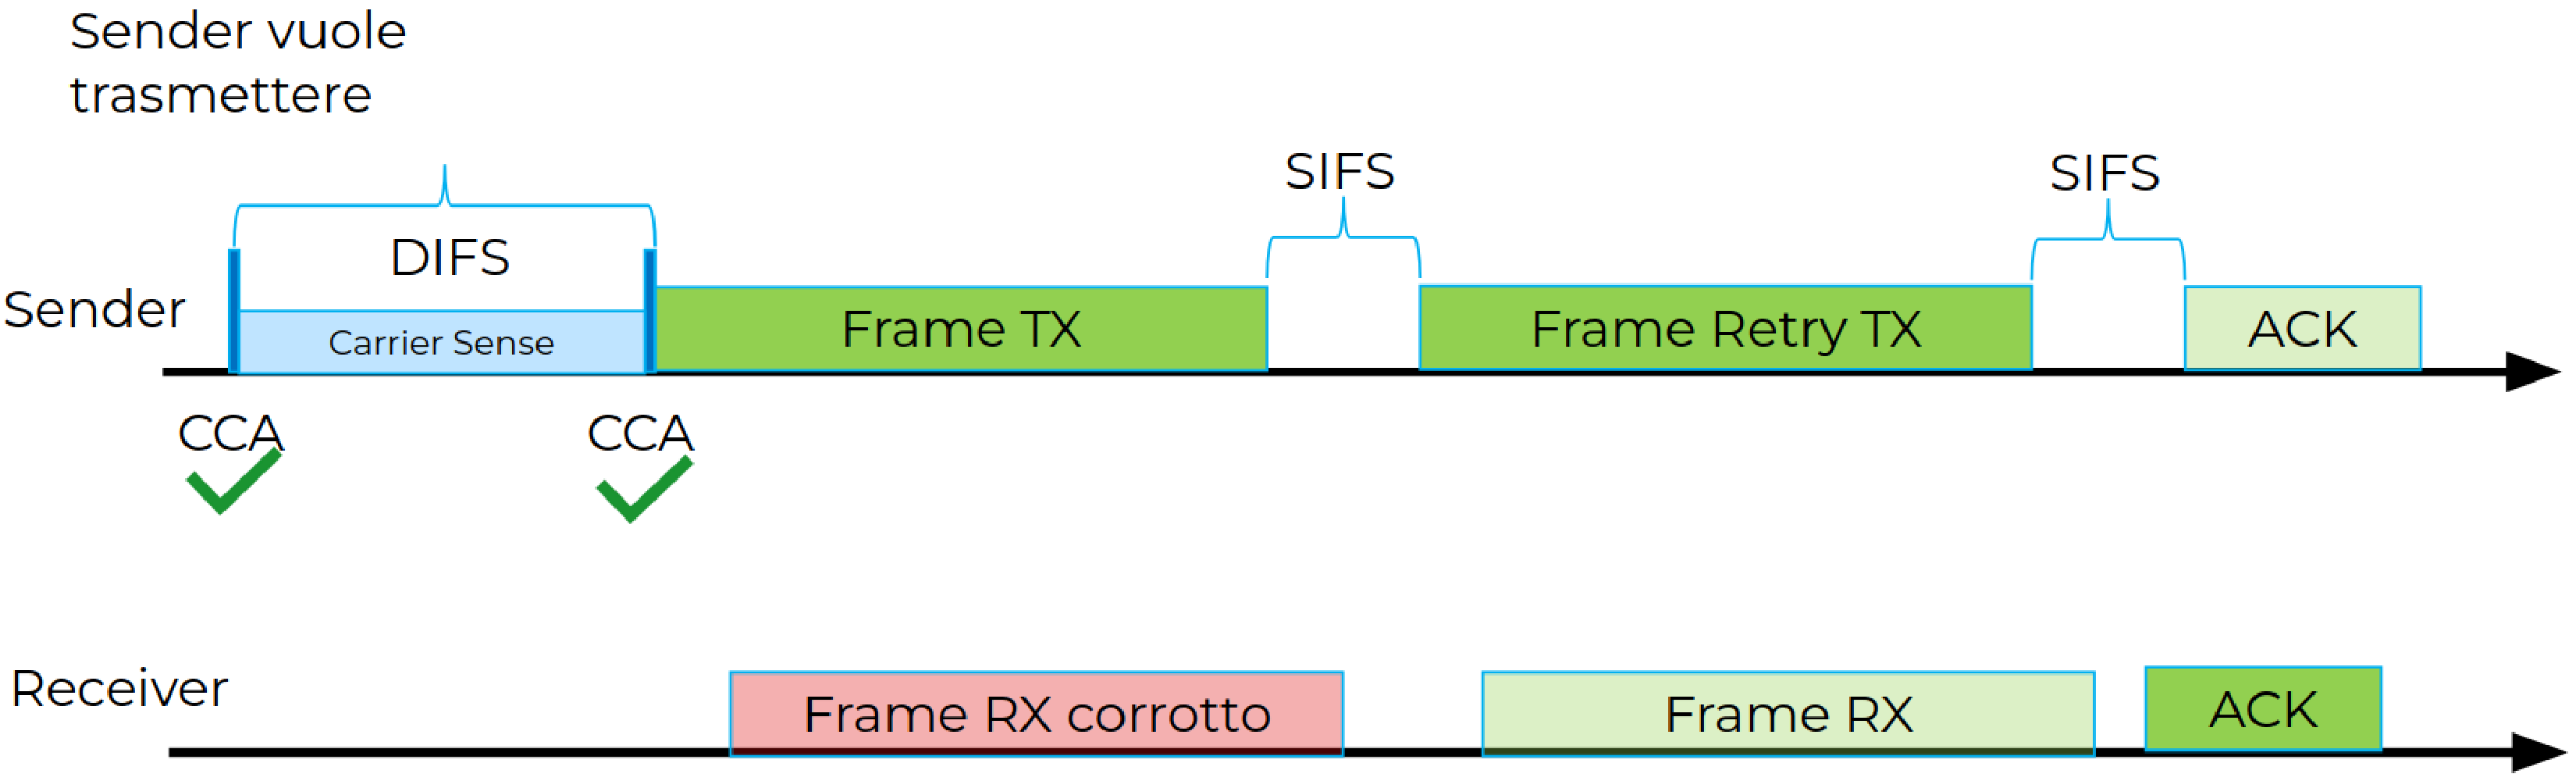
\includegraphics[width=0.98\linewidth]{img/wlan/dcfcsmaca}
\end{center}

Se il \textbf{canale è occupato}, ovvero durante il tempo di attesa DIFS viene ricevuto un segnale, fallisce il CCA ed il dispositivo ascolta fino al termine della trasmissione dell'altro sender.\\

Quando il canale è di nuovo libero (nuovo CCA), si aspetta un periodo di tempo DIFS, PIFS o SIFS, deciso in base alla priorità del messaggio, prima di avere un periodo di contesa (tutti i dispositivi che devono trasmettere aspettano il momento di fine trasmissione).\\
Durante il periodo di contesa il dispositivo aspetta un numero random di slot\_time da attendere (Binary Exponential Backoff). Carrier sense durante tutto il priodo di backoff.
\begin{center}
	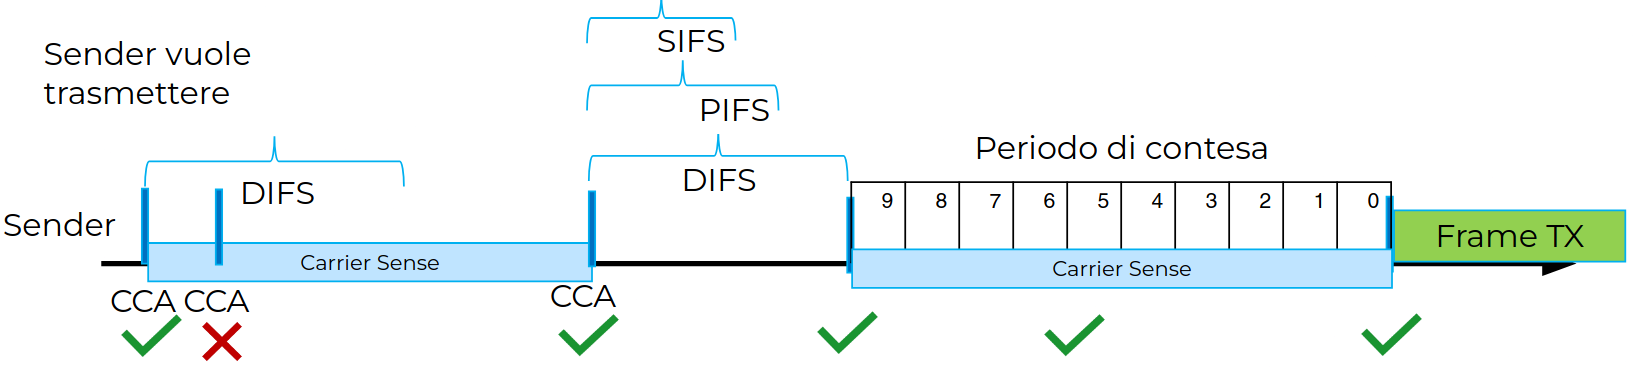
\includegraphics[width=0.98\linewidth]{img/wlan/occupied1}
\end{center}

Da notare come la radio rimanga sempre accesa, non ci sono più requisiti di batteria come in Bluetooth o ZigBee.\\

Se durante il periodo di contesa il \textbf{canale diventa occupato}, due opzioni:
\begin{enumerate}
	\item Riparto dalla contesa (con intervallo più ampio) al prossimo ciclo; non equa nei confronti delle stazioni che hanno "perso", rischio attesa infinita
	\item Blocco il timer al valore in cui era arrivato nel momento in cui è stato rilevato il canale occupato e nel \textbf{turno successivo riparto} da quel valore
\end{enumerate}

%DoS?

\newpage

\subsubsection{Problema del terminale nascosto}

Il meccanismo di carrier sense funziona se l'altro dispositivo che comincia a trasmettere può essere rilevato. Ad esempio, nel caso
\begin{center}
	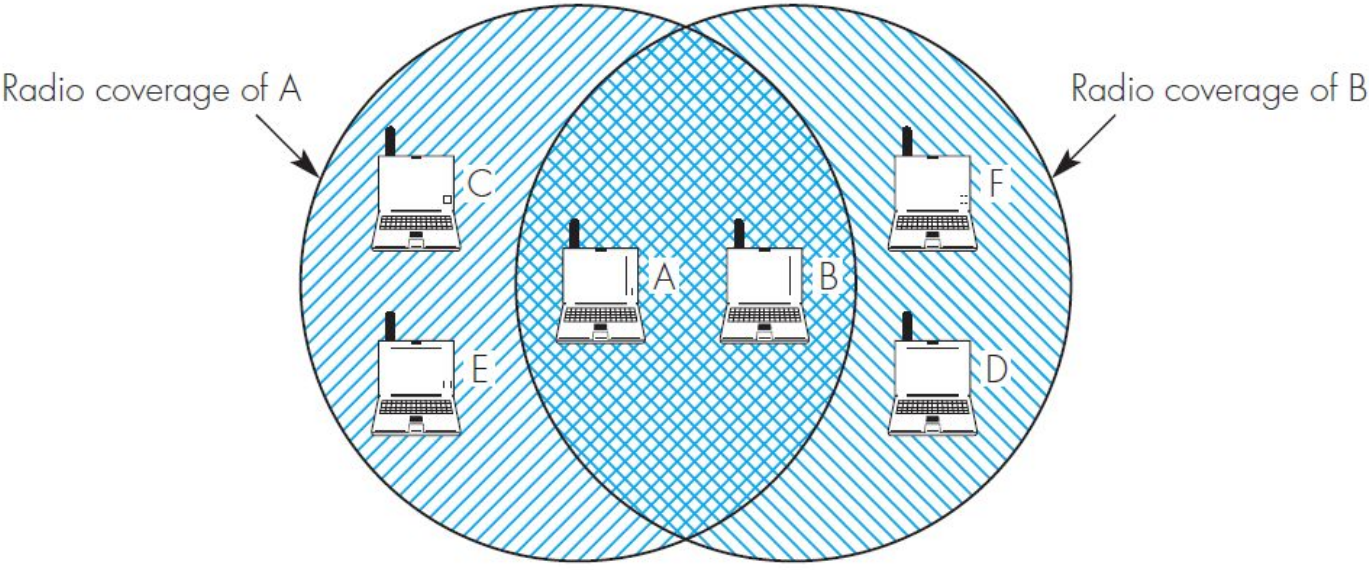
\includegraphics[width=0.6\linewidth]{img/wlan/sneaky}
\end{center}
A e D non si possono sentire in quanto fuori dal rispettivo raggio di copertura. Se entrambi volessero trasmettere a B vedrebbero il canale libero nello stesso momento, causando una collisione.
\begin{center}
	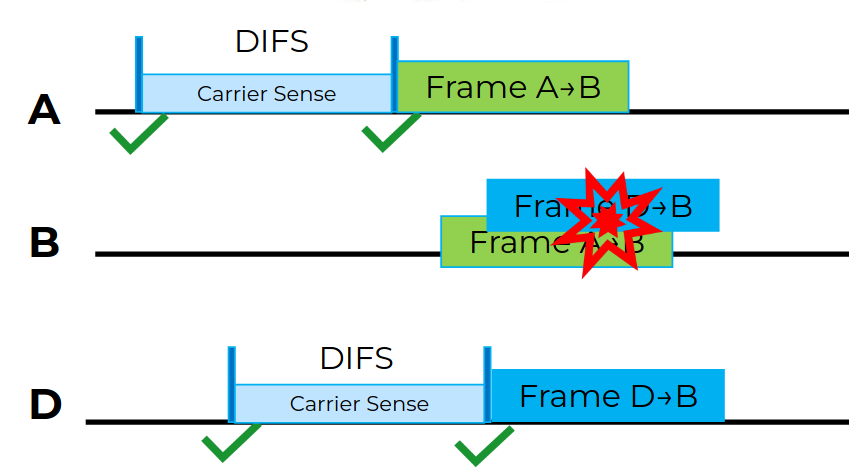
\includegraphics[width=0.55\linewidth]{img/wlan/boom}
\end{center}